\documentclass[11pt,a4paper]{article}
\usepackage[margin=2.1cm]{geometry}
\usepackage{amsmath,booktabs,tabularx,xcolor,hyperref,enumitem,graphicx,float}
\hypersetup{colorlinks,linkcolor=blue!50!black,urlcolor=blue!50!black}
\setlist{itemsep=1pt,topsep=2pt}
\newcommand{\code}[1]{\texttt{\small #1}}
\definecolor{bad}{HTML}{B5403A}\definecolor{good}{HTML}{2E7D4F}

\title{Does the fair line beat the widest bonds?\\[2pt]\large A backtest of the Section 7.5 alpha forecast, 2008--2026}
\author{FundamentalQuantmental, HY Analyst}
\date{TRACE month ends January 2008 to August 2026; run 22 October 2026}

\begin{document}
\maketitle

\noindent\fcolorbox{gray}{gray!6}{\parbox{\dimexpr\linewidth-2\fboxsep-2\fboxrule}{%
\textbf{The answer}
\begin{enumerate}
\item \textbf{\color{bad}No. The fair line does not beat ``buy the widest''.} Rank IC after cost at 3 months: widest 0.22 ($t$ 6.8), fair line after cost 0.21 ($t$ 7.7). At 6 months: 0.29 ($t$ 6.2) against 0.25 ($t$ 6.2).
\item \textbf{The leverage residual adds a small amount.} After we remove what spread level explains each month, the convergence term still has an IC of 0.036 ($t$ 2.2) at 3 months. Real, but small.
\item \textbf{\color{bad}The size is wrong.} Calibration slope (Mincer--Zarnowitz $b$) is 0.07 (se 0.05) at 3 months. A predicted 100 bp earns about 7 bp. In 2019--2026 alone the slope is 0.3: still three times too confident.
\item \textbf{\color{good}The cycle bar passes, with a caveat.} IC after cost is positive in all four cycle windows (2008--09, 2015--16, 2020, 2022) for every rule. But in calendar years 2008 and 2015 the IC is negative for every rule. The recovery years carry the windows.
\item \textbf{\color{bad}After cost, the long-short does not compound.} Top minus bottom decile, fair line, 3 months: mean $+5.3\%$ a year ($t$ 0.8), compounded $-0.9\%$ a year, worst drawdown $-65\%$.
\item \textbf{\color{bad}The two-clocks signals add nothing beyond spread.} More years of fixed charges go with more spread (as expected) and with \emph{higher}, not lower, hedged returns. After spread level is removed, the E5 IC is $-0.01$ ($t$ $-0.7$). Section~\ref{sec:clocks}.
\end{enumerate}
\textbf{What to do next.} Turn on the default-loss term (needs a PD) and the lease adjustment (needs XBRL). Then rerun this test. Until then, the model ranks about as well as spread alone and must not size positions.}}

\section*{What ``good'' looks like}
\begin{enumerate}
\item \textbf{Ranking:} the rank IC is above zero, with a $t$-statistic above 2 after the overlap correction.
\item \textbf{Size:} the slope $b$ of realised on predicted alpha is near 1, and the intercept $a$ is near 0.
\item \textbf{Beats the benchmark:} the IC is higher than the IC of the widest rule on the same bonds.
\item \textbf{Survives stress:} the IC after cost is positive in at least three of the four cycles.
\end{enumerate}

\section{Method in seven steps}
\begin{enumerate}
\item \textbf{Build the universe each month with no look-ahead.} Take every TRACE bond whose master record \emph{at that month end} says grade H, fixed coupon, not convertible. Price it from trades of \$100k par or more in the last 7 days of the month (par-weighted). Remove cancels and corrections in all three TRACE code eras. Compute the G-spread from the Treasury par curve of that day.
\item \textbf{Keep the bonds that die.} A bond that stops trading keeps one more row at its last price, then leaves. Coupon accrual stops at its last trade. A matured bond redeems at 100. 5\% of returns end this way.
\item \textbf{Link issuers and read leverage as known then.} Bond CUSIP (first six characters) to Compustat, else the TRACE ticker. Leverage $=$ (current $+$ long-term debt) $/$ LTM EBITDA from the Compustat point-in-time history, using only versions published by the month end.
\item \textbf{Predict at month end $t$ with data known at $t+1$ day.} Four rules (below). A guard stops any input row with \code{available\_at} after the decision time; a test leaks one row and must fail.
\item \textbf{Measure realised alpha over $h$ = 3 and 6 months.} Hedged return of a long bond:
\[
\alpha^{real} = \underbrace{\tfrac{P_{end} - P_t + 100\,c\,\tau}{P_t}}_{\text{bond total return}} - \underbrace{\big(y^T_t \tau - D\,\Delta y^T\big)}_{\text{matched Treasury}} - \beta\underbrace{\big(S_t \tau - D\,\Delta S\big)}_{\text{HY benchmark spread}} \approx (s-\beta S)\tau - D(\Delta s - \beta\,\Delta S).
\]
$D$ is modified duration, $S$ the month's median G-spread of the high yield market, $\beta = 1$.
\item \textbf{Subtract cost.} Round trip $=$ one bid-ask spread over price. Proxy: dealer-sell minus dealer-buy price to customers (from about 2012), else the intraday high-low. Median 24 bp of price.
\item \textbf{Score.} Monthly Spearman IC; Newey--West $t$ with $h-1$ lags (the horizons overlap). Pooled regression $\alpha^{real} = a + b\,\hat\alpha$ with Driscoll--Kraay errors. Decile long-short after cost. PIT of realised against $N(\hat\alpha, \sigma_t)$, with $\sigma_t$ from completed past errors.
\end{enumerate}

\subsection*{The four rules}
\begin{center}
\begin{tabularx}{\linewidth}{@{}lX@{}}\toprule
Rule & Predicted alpha $\hat\alpha$ \\\midrule
\code{widest} & G-spread $s$. The benchmark: buy what pays most. \\
\code{fair\_conv} & $D\,(1-\rho^{h})\,(s - s^{fair})$, with $s^{fair} = s\,e^{-\varepsilon}$ and $\varepsilon$ the issuer residual of $\log s_{5y} = a + b\cdot\text{leverage}$, fitted each month across issuers. \\
\code{fair\_line} & $(s - \beta S)\,h/12 + $ \code{fair\_conv}: the Section 7.5 alpha without macro paths and without the loss term. \\
\code{fair\_line\_net} & \code{fair\_line} minus the round-trip cost. \\\bottomrule
\end{tabularx}
\end{center}
$\rho$ is one monthly AR(1) slope pooled over all issuers' past residuals (expanding window). Fitted value: 0.91 to 0.95 a month (half-life 8 to 14 months). The fair-line slope $b$ is small: median 0.055 per turn (one more turn of leverage adds about 6\% to the spread).

\section{Results}
\subsection*{Ranking and size, all four rules, same bonds}
\begin{center}
{\small\begin{tabular}{@{}llrrrrrr@{}}\toprule
 & & \multicolumn{3}{c}{Rank IC} & & \multicolumn{2}{c}{Long-short after cost, a year} \\
$h$ & Rule & gross & net & $t$ (net) & MZ $b$ (se) & mean & compounded \\\midrule
3 & widest        & 0.266 & 0.225 & 6.8 & 0.27 (0.12) & $+7.1\%$ & $+1.4\%$ \\
3 & fair\_conv    & 0.184 & 0.159 & 6.0 & 0.04 (0.04) & $+3.6\%$ & $-2.1\%$ \\
3 & fair\_line    & 0.213 & 0.183 & 6.5 & 0.07 (0.05) & $+5.3\%$ & $-0.9\%$ \\
3 & fair\_line\_net & 0.201 & 0.210 & 7.7 & 0.06 (0.05) & $+4.6\%$ & $-1.2\%$ \\\midrule
6 & widest        & 0.322 & 0.295 & 6.2 & 0.56 (0.26) & $+9.8\%$ & $+2.6\%$ \\
6 & fair\_conv    & 0.224 & 0.208 & 5.5 & 0.05 (0.04) & $+7.5\%$ & $+0.8\%$ \\
6 & fair\_line    & 0.260 & 0.241 & 5.9 & 0.08 (0.06) & $+8.7\%$ & $+1.5\%$ \\
6 & fair\_line\_net & 0.254 & 0.251 & 6.2 & 0.08 (0.05) & $+8.5\%$ & $+1.4\%$ \\\bottomrule
\end{tabular}}
\end{center}
\noindent IC net scores each rule against realised alpha minus the bond's own round-trip cost. The MZ slope of \code{widest} is in spread units, not return units; read it only as a sign. \code{fair\_line\_net} has a higher IC net than gross because its cost term also sits in the net return: part of that gain is mechanical.

\subsection*{The cycle test (IC after cost, mean over formation months in the window)}
\begin{center}
\begin{tabular}{@{}llrrrrc@{}}\toprule
$h$ & Rule & 2008--09 & 2015--16 & 2020 & 2022 & Cycles positive \\\midrule
3 & widest         & 0.184 & 0.237 & 0.392 & 0.089 & 4 of 4 \\
3 & fair\_line\_net & 0.189 & 0.192 & 0.276 & 0.134 & 4 of 4 \\
6 & widest         & 0.237 & 0.291 & 0.569 & 0.149 & 4 of 4 \\
6 & fair\_line\_net & 0.220 & 0.220 & 0.417 & 0.162 & 4 of 4 \\\bottomrule
\end{tabular}
\end{center}
By calendar year, 2008 ($-0.09$ to $-0.17$) and 2015 ($-0.07$ to $-0.13$) are negative for both rules. In the sell-off the wide bonds got wider; they paid back in the recovery. The fair line loses less than widest in those years, and gains more in 2022.

\subsection*{Robustness}
\begin{enumerate}
\item \textbf{Skip a month} between the signal and the return: every IC falls by about 0.02; the order of the rules does not change. Bid-ask bounce does not drive the result.
\item \textbf{Issuers linked by CUSIP only} (63\% of scored bond-months): ICs within 0.01 of the full set.
\item \textbf{Pilot 2019--2026:} same order of rules; MZ slope 0.25--0.31; IC after cost 0.21 (fair line) against 0.25 (widest) at 3 months.
\item \textbf{Beyond spread:} IC of \code{fair\_conv} against realised alpha net of a per-month fit on the spread rank: 0.036 ($t$ 2.2) at 3 months, 0.048 ($t$ 1.9) at 6 months.
\item \textbf{PIT:} 75--80\% of outcomes fall in the middle two deciles, and only 2--3\% in each outer decile (uniform: 10\% each). The errors are peaked with long tails. A normal band whose width is set by the tails is too wide for most bonds.
\end{enumerate}


\section{The two-clocks signals (Section 4.7, estimate E5)}\label{sec:clocks}
\textbf{Answer.} No clock signal predicts hedged excess return beyond spread level. The fixed-charge measure has the expected link to spread, but its return IC has the opposite sign to the memo's use, and spread explains all of it.

\subsection*{How the signals are built, in five steps}
\begin{enumerate}
\item \textbf{Read every 10-K and 10-Q from SEC companyfacts.} Map each scored issuer to its CIK through Compustat. Keep the lease, debt, and purchase-obligation maturity tags, the balance-sheet debt tags, and \code{RevenueRemainingPerformanceObligation}.
\item \textbf{Build the clocks with the existing code.} Each filing becomes an undimensioned instance table. \code{schedules.ladder}, \code{reconcile\_debt}, \code{clocks.ladder}, \code{tail\_years\_run\_rate}, \code{clocks.rpo}, and \code{clocks.mismatch} run unchanged. Rolling-year and newer purchase names map to the names \code{schedules} knows. A missing year inside a ladder counts as zero (11\% of filings).
\item \textbf{Keep it point in time.} A filing's clocks are known from its filing date $+$ 1 day. A filing that omits a ladder takes the last one (at most 400 days old), aged to its date, as \code{clock\_case} does.
\item \textbf{Form three signals at each month end,} signed as the combined score uses them (higher $=$ less clock risk):
\begin{gather*}
e_5 = -\frac{\text{fixed obligations}}{\text{LTM EBITDA} + \text{first-year rent}},\\
dgap = -(\text{duration gap}),\qquad renew = -(\text{renewal-dependent share}).
\end{gather*}
EBITDA and revenue come from Compustat point in time. $renew$ counts only where RPO is at least 25\% of LTM revenue. Where a filing tags no debt, Compustat debt is added (5\% of issuer-months).
\item \textbf{Score each signal like the alpha rules,} on the same bonds: IC after cost, IC beyond spread level (\code{backtest.ic\_beyond}), and the 2020 and 2022 cycles.
\end{enumerate}

\subsection*{Results, formation months 2018-01 to 2026-08}
{\small
\begin{tabular}{@{}llrrrrrrr@{}}\toprule
 & & \multicolumn{2}{c}{IC after cost} & \multicolumn{2}{c}{IC beyond spread} & \multicolumn{2}{c}{Cycles (IC after cost)} & Widest, \\
$h$ & Signal & mean & $t$ & mean & $t$ & 2020 & 2022 & same bonds \\\midrule
3 & $e_5$   & $-0.082$ & $-4.5$ & $-0.011$ & $-0.7$ & $-0.159$ & $-0.020$ & 0.237 \\
3 & $dgap$  & $+0.010$ & $0.7$  & $+0.015$ & $1.2$  & $+0.001$ & $+0.051$ & 0.253 \\
3 & $renew$ & $-0.015$ & $-0.9$ & $-0.021$ & $-1.4$ & $-0.048$ & $+0.018$ & 0.239 \\\midrule
6 & $e_5$   & $-0.114$ & $-4.7$ & $-0.032$ & $-1.2$ & $-0.224$ & $-0.060$ & 0.305 \\
6 & $dgap$  & $+0.002$ & $0.1$  & $+0.015$ & $1.0$  & $-0.046$ & $+0.045$ & 0.342 \\
6 & $renew$ & $-0.032$ & $-1.3$ & $-0.035$ & $-1.8$ & $-0.073$ & $-0.007$ & 0.318 \\\bottomrule
\end{tabular}}

\begin{enumerate}
\item \textbf{The expected sign holds for spread.} Rank correlation of fixed-charge years with G-spread: $+0.32$ ($t$ 36). The market prices the clock.
\item \textbf{The return sign is the opposite of E5.} Bonds with more years of fixed charges earned \emph{more} after the hedge ($e_5$ IC $-0.08$). That is carry: they pay more spread. With spread removed, the IC is $-0.01$ ($t$ $-0.7$) at 3 months and $-0.03$ ($t$ $-1.2$) at 6 months: no information beyond spread, in either direction.
\item \textbf{The cycle check fails.} $e_5$ is negative in both covered cycles. $dgap$ is positive in both at 3 months, but its full-sample IC is 0.01 ($t$ 0.7).
\item \textbf{Decision for the combined score:} keep E5 out of the alpha estimate (weight 0), keep the clocks as risk measures in the pair report (S9). The measure is real; the market already prices it.
\end{enumerate}

\begin{figure}[H]\centering
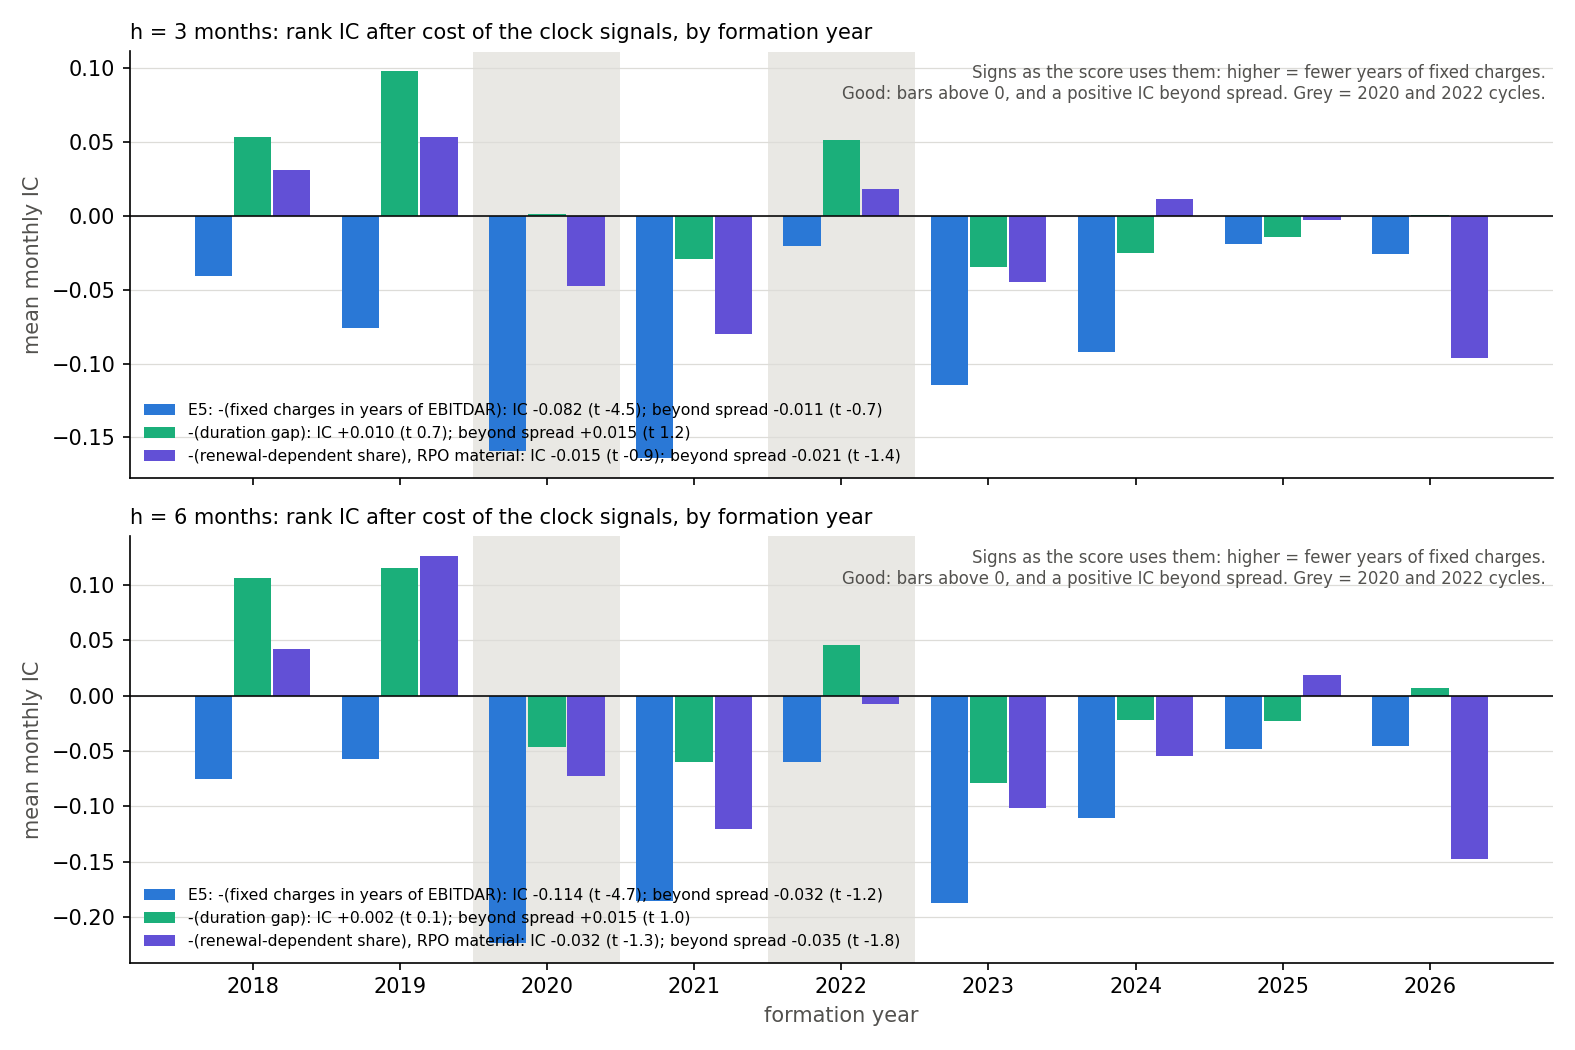
\includegraphics[width=\linewidth]{figures/backtest_clocks_full.png}
\caption{Rank IC after cost of the three clock signals by formation year. Signs as the score uses them. Good: bars above zero and a positive IC beyond spread. $e_5$ (blue) is below zero in every year: high-charge issuers earn their extra spread. Grey: the 2020 and 2022 cycles.}
\end{figure}

\subsection*{Coverage}
\begin{center}
\begin{tabularx}{\linewidth}{@{}lX@{}}\toprule
Scored issuers since 2018 & 1,408; with a CIK 1,396; with companyfacts ladders 1,178 \\
Filings read & 53,781 (14\% tag RPO) \\
$e_5$ & 1,143 issuers, 7,001 bonds, 103 months, median 1,334 bonds a month \\
$dgap$ (RPO tagged) & 343 issuers, median 241 bonds a month \\
$renew$ (RPO material) & 187 issuers, median 110 bonds a month \\
SEC pull & 1,396 documents in 3.8 minutes, no failures; clock build 25 minutes \\\bottomrule
\end{tabularx}
\end{center}

\subsection*{Limits of the clock test}
\begin{enumerate}
\item \textbf{No RPO timing.} Companyfacts drops the dimensional timing facts, so every RPO burns evenly over 2 years (the \code{clock\_inputs} default). The duration gap is then the obligation duration less 1 year, and the renewal share is the share of obligations after year 2. The revenue clock adds no issuer-specific timing.
\item \textbf{Obligations are partial.} No interest (no rate in the feed), no leases not yet commenced (dimensional). Fixed charges are therefore a floor. 50\% of filings carry at least one ladder from an earlier filing.
\item \textbf{Short history.} ASC 842 and 606 start in 2018--2019, so only the 2020 and 2022 cycles are covered. The CLAUDE.md bar (3 of 4 cycles) cannot be met by construction.
\item \textbf{Filing date, not acceptance time.} Companyfacts gives the date only. We add one day, which can lag the market by up to a day.
\end{enumerate}

\section{Figures}
\begin{figure}[H]\centering
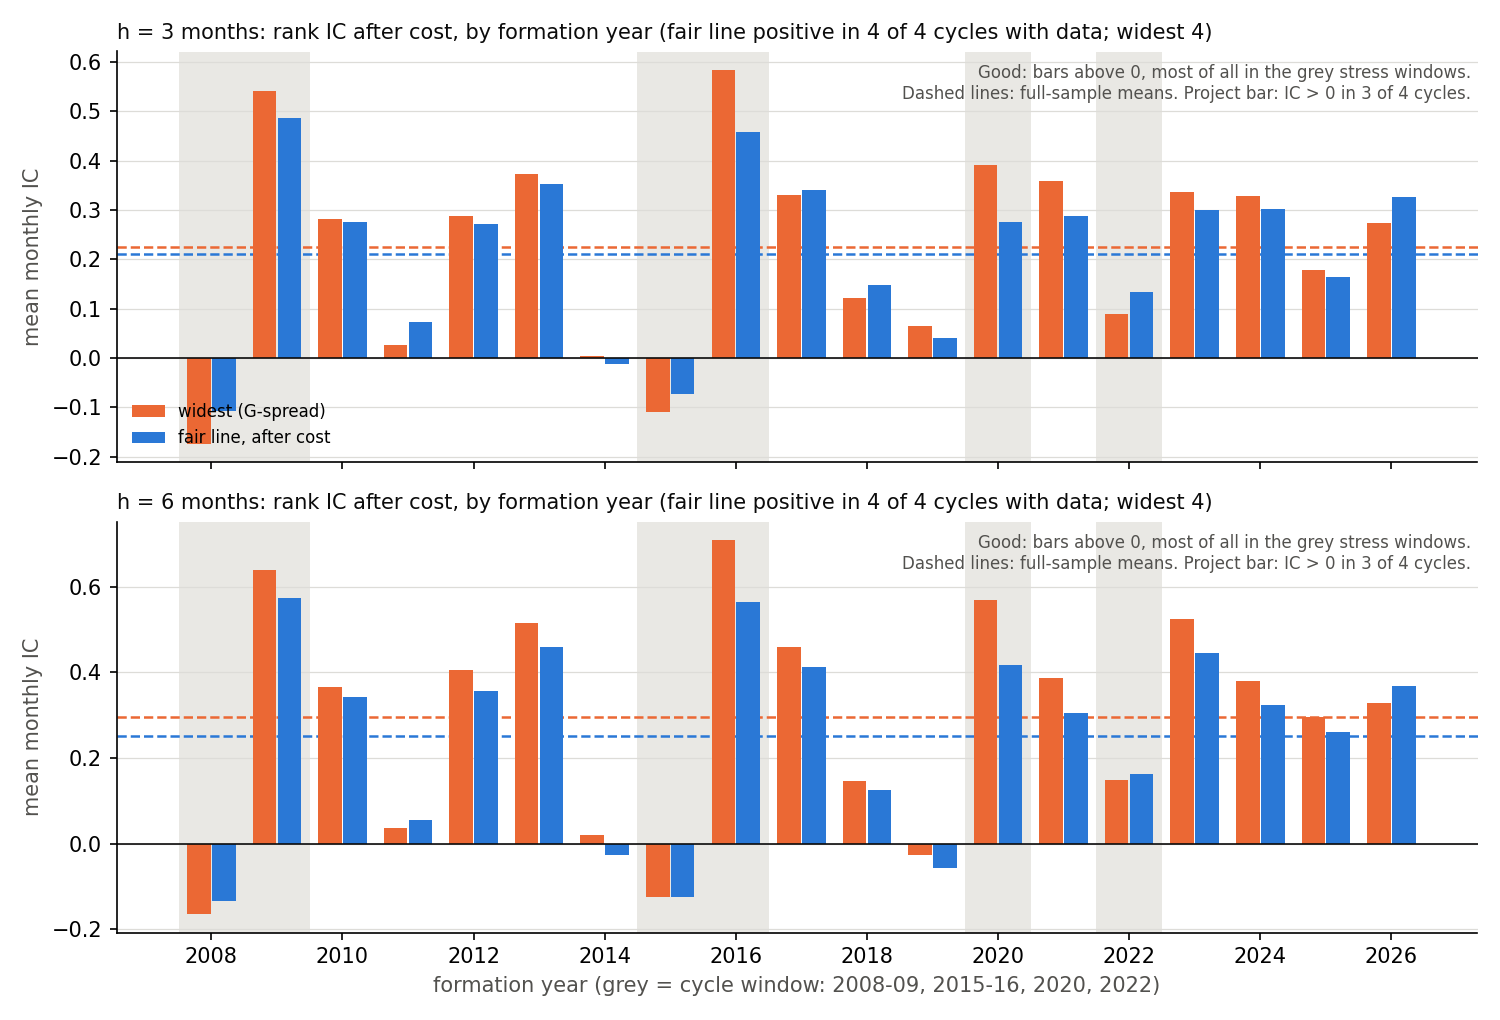
\includegraphics[width=\linewidth]{figures/backtest_ic_by_year_full.png}
\caption{Rank IC after cost by formation year. Grey: the four cycle windows. Good: bars above zero, most of all in grey. Both rules fail in 2008 and 2015 and recover the next year. The fair line (blue) does not beat widest (orange) in most years.}
\end{figure}
\begin{figure}[H]\centering
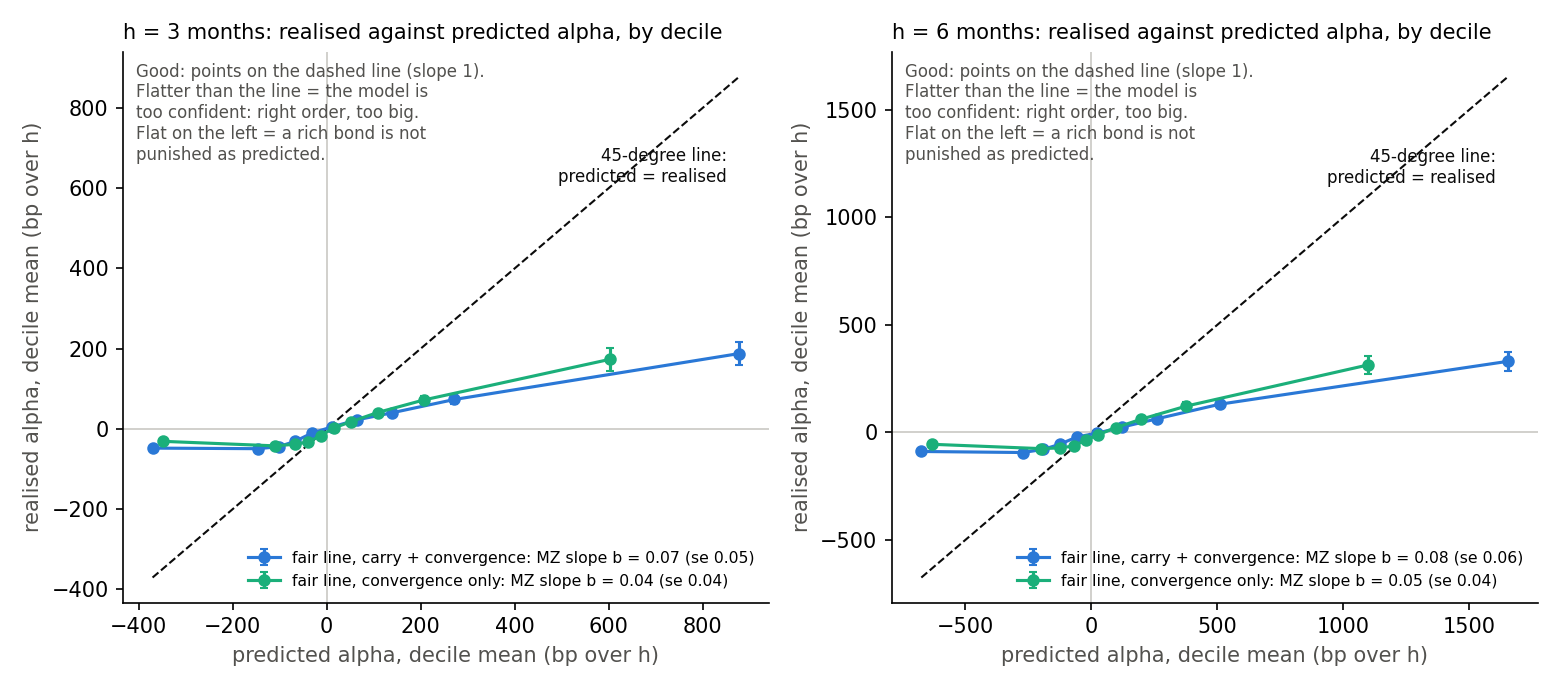
\includegraphics[width=\linewidth]{figures/backtest_calibration_full.png}
\caption{Calibration by decile of predicted alpha. Good: points on the dashed 45-degree line. The points lie on a line about one third as steep in the middle and flatten in the tails: right order, far too big. On the left, rich bonds are not punished as predicted.}
\end{figure}
\begin{figure}[H]\centering
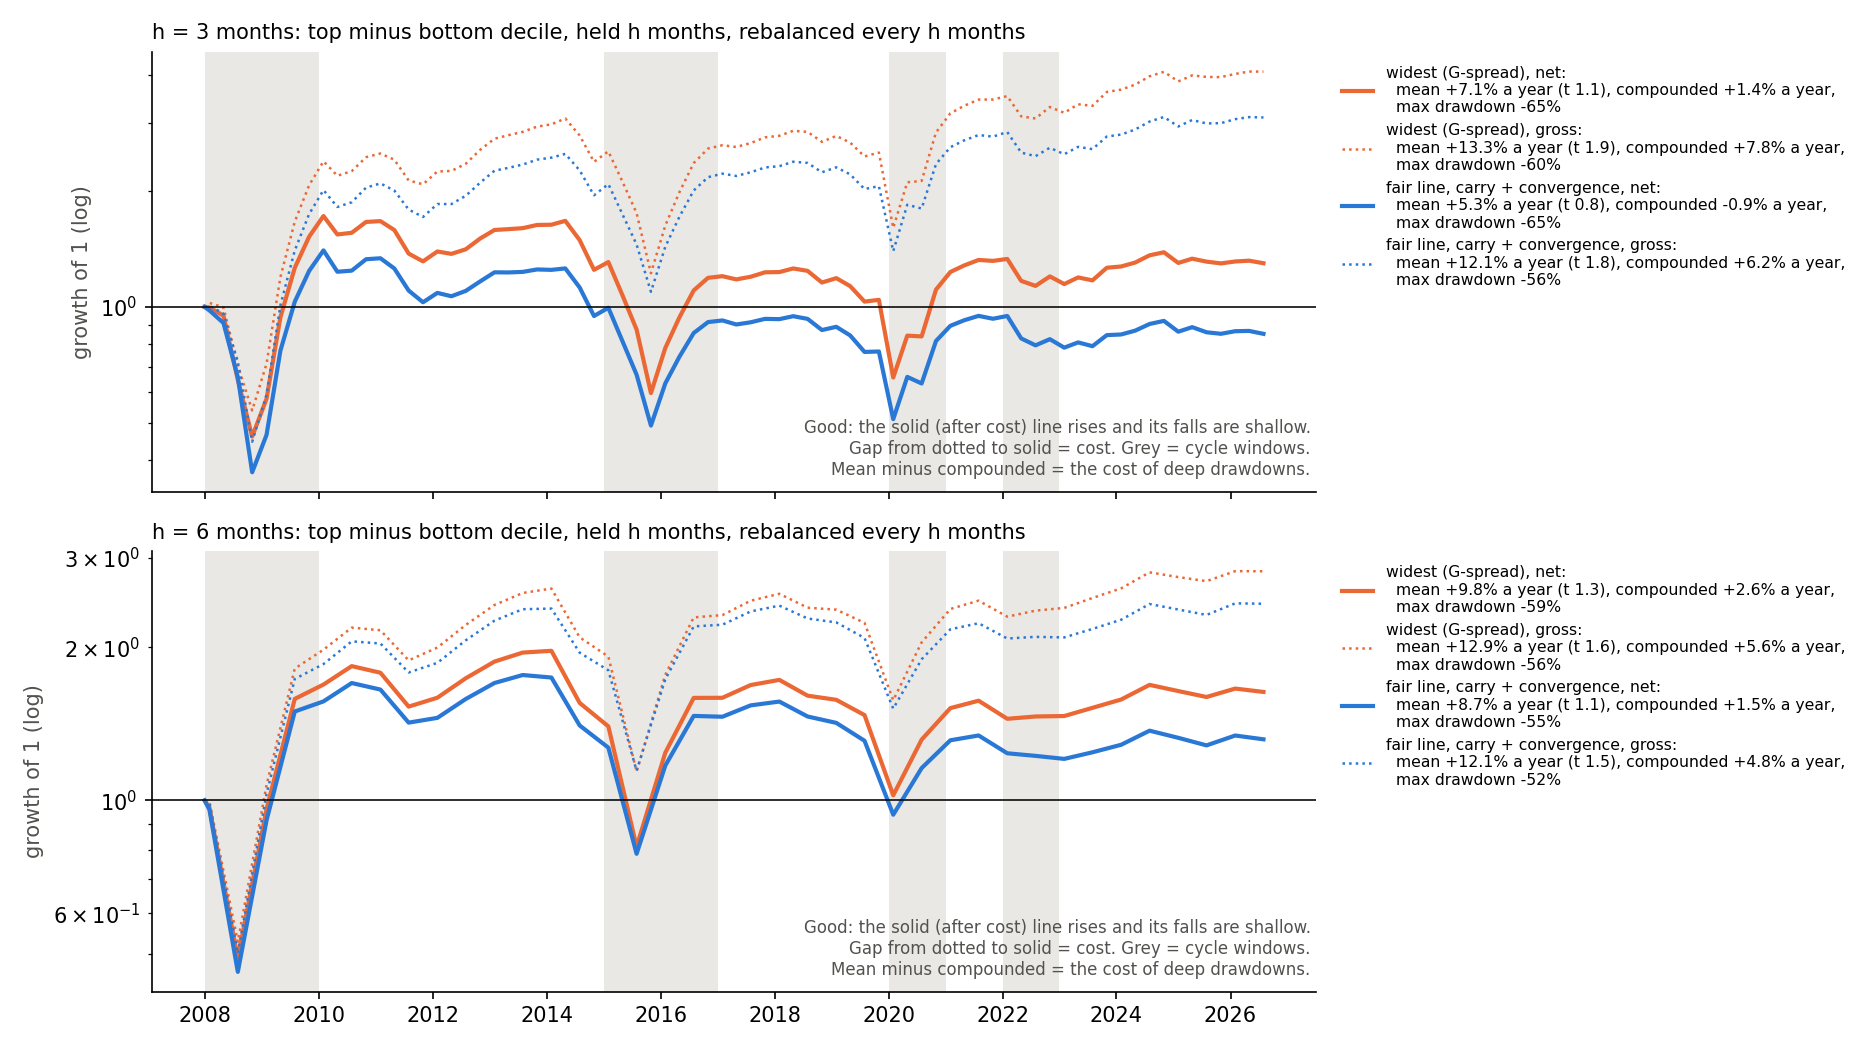
\includegraphics[width=\linewidth]{figures/backtest_long_short_full.png}
\caption{Top minus bottom decile, non-overlapping holds, growth of 1 on a log scale. Dotted: before cost. Solid: after cost. The gap is cost. The deep falls in 2008, 2015 and 2020 are the wide bonds in stress; they erase most of the mean.}
\end{figure}

\section{Data coverage}
\begin{center}
\begin{tabular}{@{}lr@{}}\toprule
Months & 224 (2008-01 to 2026-08) \\
Bonds in the TRACE grade-H panel & 34,542 (706,287 bond-months) \\
Issuer keys linked to Compustat & 49\% (CUSIP 2,579; ticker 4,436; none 7,249) \\
Eligible bond-months with leverage & 48\% \\
Scored set (all four rules present) & 13,271 bonds, 1,964 issuers, 287,720 bond-months \\
Bonds per month in the scored set & median 1,430, minimum 258 \\
Bid-ask proxy source & side 45\%, day range 38\%, month median 17\% \\
TRACE pulls (WRDS, 3 connections) & 92 months in 21 min, 132 months in 19 min \\\bottomrule
\end{tabular}
\end{center}

\section{Limits, largest first}
\begin{enumerate}
\item \textbf{No default-loss term.} No PD is in the panel, so the forecast ignores expected loss. The widest decile holds the defaults; this is the most likely cause of the flat calibration slope.
\item \textbf{Leverage only, no lease adjustment, half the issuers.} The Compustat point-in-time history has no lease field. Only 49\% of issuer keys link; 38\% of the scored set links by ticker, which can hit a reused ticker. The point-in-time history ends in February 2026, so the 2026 fair line thins to about 200 issuers.
\item \textbf{Duration ignores calls.} Most high yield bonds are callable. Modified duration to maturity overstates the rate and spread hedge for bonds above par; this shifts the level of realised alpha (mean $-0.8\%$ a quarter in 2019) more than its rank.
\item \textbf{Cost is a proxy.} Before 2012 TRACE has no trade side, so the intraday high-low range sets the cost. It overstates the spread when the price moves inside the day.
\item \textbf{Crossover names.} Grade H in TRACE includes split-rated and recently downgraded bonds. Without ratings we cannot take them out or rating-match the benchmark.
\item \textbf{Thin early sample.} Before mid-2014 TRACE does not disseminate 144A trades; the 2008--2013 panel has about 1,200 bonds a month.
\end{enumerate}

\section{Reproduce}
\begin{center}\footnotesize\texttt{PYTHONPATH=. python3 scripts/backtest\_alpha.py --start 2008-01 --end 2026-08 --tag full}\end{center}
A cached run takes 5 minutes.
\begin{itemize}
\item Results: \code{data/raw/backtest/summary\_full.json}.
\item Tests: \code{tests/test\_backtest.py} and \code{tests/test\_trace\_panel.py}.
\item Design: \code{docs/decisions/2026-10-22-alpha-backtest-design.md}.
\end{itemize}

\end{document}
